\documentclass[border=10pt]{standalone}

\usepackage{tikz}
\usepackage{tikzsymbols}
\usetikzlibrary{calc,patterns,shapes.geometric}

\def\centerarc[#1](#2)(#3:#4:#5){\draw[#1] ($(#2)+({#5*cos(#3)},{#5*sin(#3)})$) arc (#3:#4:#5);}

\begin{document}
	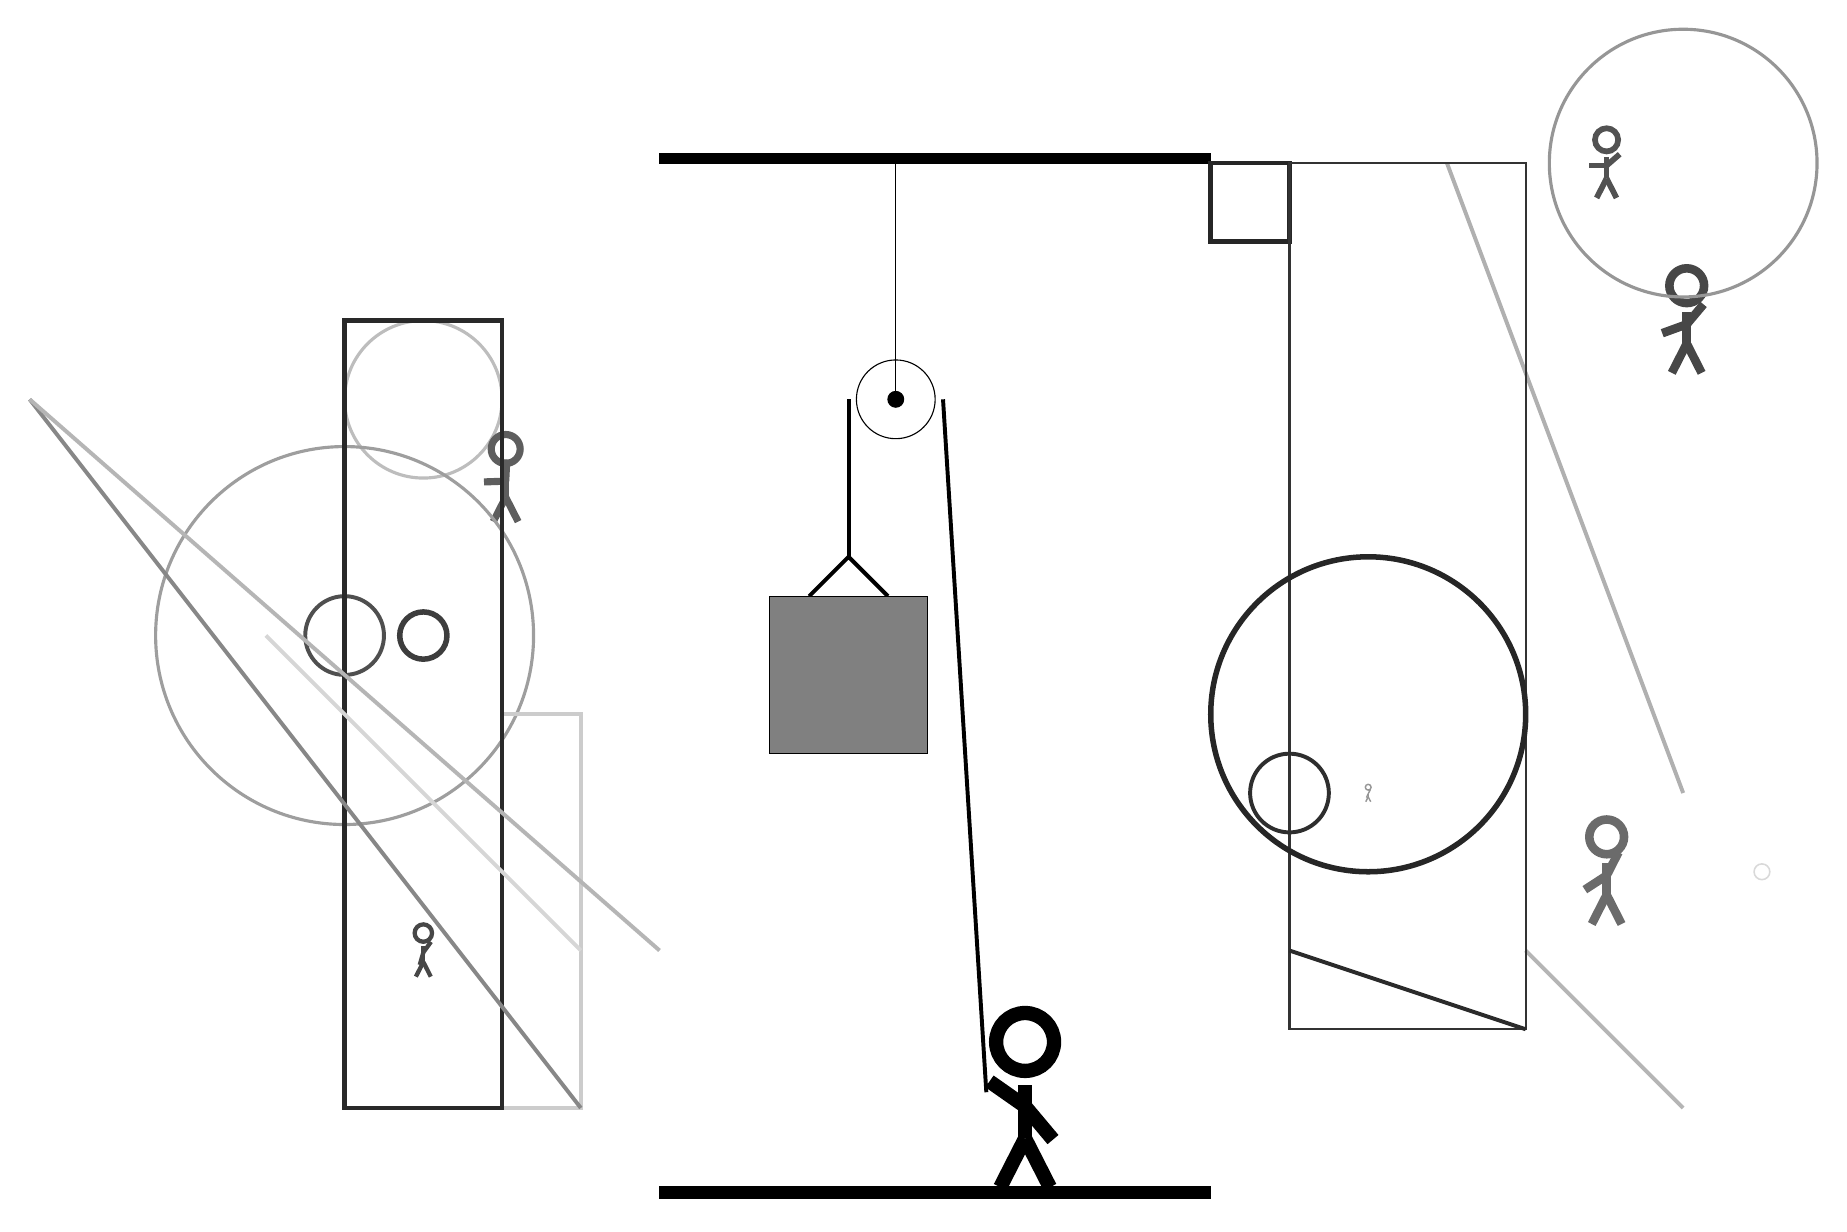
\begin{tikzpicture}
		%%%%% START %%%%%
		
		\draw[fill=black] (-2, 10) rectangle (5, 10.125);
		
		\draw [line width=0.7mm, color=black!76](-5, 4) circle (0.3);
		
		\draw [line width=0.4mm, color=black!26](-5, 7) circle (1.0);
		\node[line width=0.6mm, color=black!63] at (-4, 6) {\Strichmaxerl[5][2][87]};
		\node[line width=0.2mm, color=black!41] at (7, 2) {\Strichmaxerl[1][66][62]};
		\draw [line width=0.2mm, color=black!15](12, 1) circle (0.1);
		\draw [line width=0.5mm, color=black!69](-6, 4) circle (0.5);
		
		\draw[line width=0.5mm, color=black!29](9, 0) -- (11, -2);
		\draw[line width=0.5mm, color=black!31](8, 10) -- (11, 2);
		\node[line width=0.6mm, color=black!72] at (11, 8) {\Strichmaxerl[6][20][50]};
		\draw [line width=0.4mm, color=black!38](-6, 4) circle (2.4);
		\draw[line width=0.6mm, color=black!85] (6, 10) rectangle (5, 9);
		
		\node[line width=0.5mm, color=black!72] at (-5, 0) {\Strichmaxerl[3][74][54]};
		\draw[line width=0.5mm, color=black!20] (-4, -2) rectangle (-3, 3);
		\node[line width=0.7mm, color=black!58] at (10, 1) {\Strichmaxerl[6][33][63]};
		\draw[line width=0.3mm, color=black!80] (6, -1) rectangle (9, 10);
		\draw [line width=0.4mm, color=black!41](11, 10) circle (1.7);
		
		\draw [line width=0.5mm, color=black!82](6, 2) circle (0.5);
		
		\node[line width=0.3mm, color=black!68] at (10, 10) {\Strichmaxerl[4][0][41]};
		\draw [line width=0.7mm, color=black!85](7, 3) circle (2.0);
		\draw[line width=0.5mm, color=black!83](6, 0) -- (9, -1);
		\draw[line width=0.6mm, color=black!84] (-4, 8) rectangle (-6, -2);
		
		\draw[line width=0.5mm, color=black!16](-3, 0) -- (-7, 4);
		
		\draw[line width=0.5mm, color=black!47](-3, -2) -- (-10, 7);
		\draw[line width=0.5mm, color=black!29](-2, 0) -- (-10, 7);
		
		\draw (1, 7) circle (0.5);
		\draw[fill=black] (1, 7) circle (0.1);
		\draw (1, 10) -- (1, 7);
		
		\draw[line width=0.5mm] (-0.1, 4.5) -- (0.4, 5.0) -- (0.9, 4.5);
		\draw[fill=black!50] (-0.6, 4.5) rectangle (1.4, 2.5);
		
		\draw[line width=0.5mm] (0.4, 7) -- (0.4, 5.0);
		\centerarc[line width=0.5mm](1, 7)(0:180:0.6);
		\draw[line width=0.5mm](1.6, 7) -- (2.15, -1.8);
		
		\node at (2.6, -1.9) {\Strichmaxerl[10][-35][-50]};
		
		\draw[fill=black] (-2, -3) rectangle (5, -3.15);
		
		%%%%% END %%%%%
	\end{tikzpicture}
\end{document}